\section{Technik}
\subsection{Auflösung}
Bei der Auflösung wird heutzutage unter SD, HD (2k), Digital Cinema (2k) und UHD (4k/8k) unterschieden. SD bedeutet Standard Definition und dominierte früher das Fernsehen. Heutzutage ist der Standard nicht mehr Standard Definiton, sondern High Definition. Obwohl bei Smartphones, TV-Geräten und Kameras schon Full-HD, also 1920 x 1080 px, der Vorreiter ist, wird zumindest im deutschen Fernsehen noch im normalen HD Format, also 1280 x 720 px, ausgestrahlt.\footnote{\label{}vgl. Jörg Jovy, 2017, S. 109f.}\newline
Bei den Videoaufnahmen wurde immer im Full-HD Format aufgenommen, also mit 1920 x 1080 px, da heutzutage die meisten Videos, von den Jugendlichen, am Smartphone angesehen werden.
\subsection{Aspect-Ratio - Seitenverhältnis}
Früher, als SD das Standard Fernsehformat war, war das Seitenverhältnis eines Fernsehbildes 4:3. Jedoch wurde später aus 4:3, 16:9, was auch heute im HD Format noch beibehalten wurde. Das SD Format verwendet rechteckige Pixel, was die Folge hat, dass ein SD Bild immer die gleiche Anzahl von Pixeln hat, nämlich 720 x 576. "Nur werden einmal rechteckige Pixel mit einem Seitenverhältnis von 1,46:1 (= 16:9) und einmal von 1,09:1 (= 4:3) verwendet." (Jörg Jovy, 2017, S.108)\newline 
Man nennt dies auch anamorph. "Anamorph bedeutet, dass die Pixel des Films nicht quadratisch sind, sondern rechteckig." (Jörg Jovy, 2017, S.572)\newline
Da Computer und HD-Bilder nur quadratische Pixel anzeigen, aber ein SD Fernsehformat rechteckige, muss man bei der Auswahl des Formats berücksichtigen, wo man das Video oder den Film schlussendlich abspielen möchte.\footnote{\label{}vgl. Jörg Jovy, 2017, S. 108, S. 572}
\subsection{Bildrate}
Seit 1967 wird im deutschen Fernsehen mit dem sogenannten PAL Format (=Phase Alternative Line) gesendet. Im PAL Format werden 25 Bilder pro Sekunde oder 50 Halbbilder pro Sekunde gesendet. Jedoch herrscht in den USA nicht das PAL Format, sondern das sogenannte NTSC Format (=National Television Systems Committee), welches 30 Vollbilder pro Sekunde oder 60 Halbbilder pro Sekunde sendet. Diese unterschiedlichen Bildraten sind der Tatsache geschuldet, da in Europa eine Wechselspannungsfrequenz von 50Hz herrscht, und in den USA eine von 60Hz.\footnote{\label{}vgl. https://gwegner.de/know-how/verwirrung-um-die-frameraten-24-fps-25-fps-30-fps-pal-ntsc-wann-nimmt-man-was/ [Zugriff: 17.03.2018]}\newline
Bei Videoaufnahmen wurde mit 25fps (= frames per second), also mit 25 Vollbildern in der Sekunde, aufgenommen.
\subsection{Farbraum}
Rot, Grün und Blau sind die drei Grundfarben des RGB Farbraums. Aus den drei Grundfarben bilden sich alle anderen Farben, die im RGB Farbraum möglich sind, was man RGB-Farbmischung nennt.\begin{quote}"Bei einer 8-Bit-Codierung pro Farbe stehen 256 verschiedene Farbwerte zur Verfügung. Aus der Mischung ergeben sich theoretisch 16,78 Mio. verschiedene Farbwerte (= 256 x 256 x 256)." (Jörg Jovy, 2017, S. 113)\end{quote} Schwarz enthält keine Farbinformation von den drei Grundfarben, wohingegen Weiß die Mischung aller drei Grundfarben ist. Der Farbraum des HD Standards ist RGB oder auch genannt als sRGB. Bei der Kamera kann zwischen sRGB und Adobe RGB umgestellt werden. Meist wird der Adobe RGB Farbraum, da er einen größeren Farbraum bietet. Wie man anhand der Abbildung \ref{fig:abb16} sehen kann, hat der Adobe RGB Farbraum mehr Grüntöne als der sRGB Farbraum.\footnote{\label{}vgl. Jörg Jovy, 2017, S. 112f.}
\begin{figure}[H]
\centering
	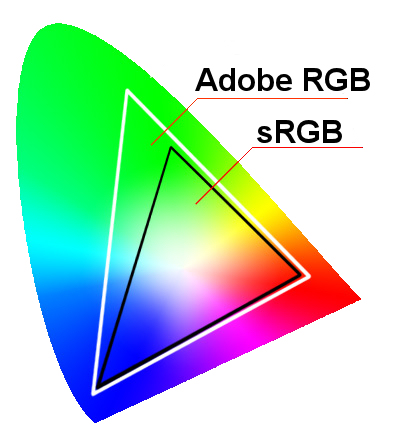
\includegraphics[width=0.3\textwidth]{abb16} 
	\caption{sRBG und Abobe RGB Farbraum}\label{fig:abb16}
\end{figure}
\subsection{Farbabtastung}
Bei der Farbabtastung handelt es sich um eine Komprimierung von  der Übertragung der Signale. Da ein unkomprimiertes Signal eine zu große Bandbreite in Anspruch nehmen würde, muss das Signal komprimiert werden. Dafür wird die Farbabtastung in Betracht gezogen. Da das menschliche Auge die Helligkeitskontraste besser auflöst als die Farbkontraste, wird bei der Farbabtastung die Helligkeit, oder Luminanz, mit der vollen Datenbreite zur Verfügung gestellt. Die Farbinformation wird, bei der Farbabtastung, jedoch reduziert. Daraus ergibt sich dann ein voll aufgelöstes Signal mit der Farbabtastung von 4:4:4. Ein bereits komprimiertes Signal hat eine Farbunterabtastung von 4:2:2, 4:2:0 oder von 4:1:1.\footnote{\label{}vgl. Jörg Jovy, 2017, S. 114.}
\paragraph{4:2:2}
\leavevmode \\
Bei der Farbunterabtastung von 4:2:2 wird bei jedem Pixel der Helligkeitswert abgetastet, wobei der Farbwert nur bei jedem zweiten Pixel abgetastet wird.\footnote{\label{}vgl. https://www.itwissen.info/Farb-Subsampling-color-subsampling.html [Zugriff: 18.03.2018]}
\paragraph{4:2:0}
\leavevmode \\
\begin{quote}"Beim Subsampling von 4:2:0, erfolgt die Abtastung der Chrominanzsignale für jeweils vier quadratisch angeordnete nebeneinander liegende Pixel. Wie bei den anderen Subsampling-Verfahren auch, wird das Luminanzsignal bei jedem Pixel abgetastet." (https://www.itwissen.info/Farb-Subsampling-color-subsampling.html [Zugriff: 18.03.2018])\end{quote}
\paragraph{4:1:1}
\leavevmode \\
Bei der Farbunterabtastung von 4:1:1 werden die Chrominanzsignale bei jeder vierter Abtastung des Helligkeitssignal abgetastet.\footnote{\label{}vgl. https://www.itwissen.info/Farb-Subsampling-color-subsampling.html [Zugriff: 18.03.2018]}
\begin{figure}[H]
	\centering	
	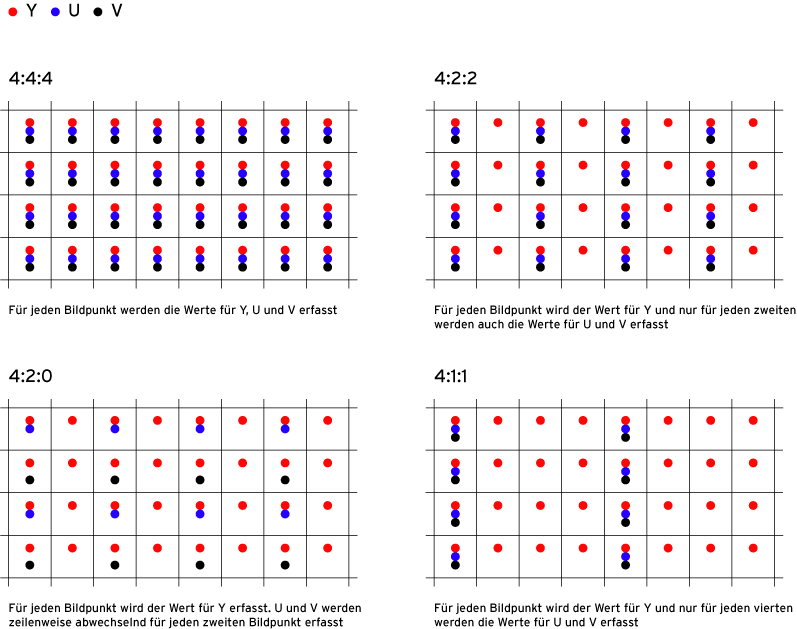
\includegraphics[width=0.8\textwidth]{abb15} 
	\caption{Farbabtastung}
\end{figure}
\subsection{Weißabgleich}
Bevor man ein Bild schießt, oder ein Video dreht, führt man zuerst einen Weißabgleich durch. Dabei wird zwischen manuellen und automatischen Weißabgleich unterschieden. Der Weißabgleich misst die derzeitige Farbtemperatur des Lichts. Die Farbtemperatur wird in Kelvin angegeben. Eine Kerze hat eine sehr rötliche und warme Farbstimmung mit einer Farbtemperatur von 1.500 Kelvin, wohingegen das Tageslicht neutral wirkt und eine Farbtemperatur von 5.000 bis 6.000 besitzt. Um den Weißabgleich manuell abzustimmen, wird ein weißes Blatt Papier vor die Kamera gehalten, und der Weißabgleich kann somit eingestellt werden. Das weiße Blatt Papier ist jedoch nur ein Hilfsmittel. Optimal wäre, eine professionelle Graukarte zu verwenden. Das Problem mit dem Papier ist, dass es optische Aufheller, die den Blauanteil erhöhen, besitzt. Das heißt, da die Kamera den zu hohen Blauanteil korrigiert, wird das Bild schlussendlich leicht gelbstichig.\footnote{\label{}vgl. Jörg Jovy, 2017, S. 201ff.}
